\documentclass[a4paper, 12pt]{scrartcl}

\usepackage{scrpage2}
\usepackage[left=2.5cm,right=2.5cm, top=3cm, bottom=4cm]{geometry}
\usepackage[utf8]{inputenc}
\usepackage[ngerman]{babel}
\usepackage[T1]{fontenc}
\usepackage{amsmath}
\usepackage{amssymb}
\usepackage{amsfonts}

\usepackage{graphicx}

\usepackage{float}
\usepackage{adjustbox}
\usepackage{hyperref}
\usepackage{textcomp}

%\usepackage{enumerate}
\usepackage[shortlabels]{enumitem}

% Einrücken verhindern
\setlength{\parindent}{0em} 


\begin{document}


\begin{titlepage}
	\centering
	{\Huge\bfseries Versuchsprotokoll\par}
	\vspace{2cm}
	{\scshape\LARGE Akustik \par}
	\vspace{1cm}
	{\Large Schallgeschwindigkeit in Festkörpern und die Physik der Gitarre\par}
	\vfill
	{\large\itshape Simon Schwarz und Marius Ising\par}

	\vfill
\end{titlepage}

\tableofcontents

\section{Schallgeschwindigkeit in Festkörpern}


\subsection{Versuchsbeschreibung}

Das Ziel des folgenden Versuchs ist die Bestimmung der Schallgeschwindigkeit und des Elastizitätsmoduls von vier verschiedenen Metallen. Das Elastizitätsmodul 
$$E = \frac{F/A}{\Delta L/L}$$
ist eine Materialkonstante und gibt die relative Längenausdehnung in Abhängigkeit von der angreifenden Zugspannung an. Eine Messung ist über die Ausbreitungsgeschwindigkeit 
$$v_l = \sqrt{\frac{E}{\rho}}$$
möglich, wobei $\rho$ die Dichte des Materials bezeichnet. Die dynamische Bestimmung von $E$ durch das direkte Messen der Längenausdehnung ist bei Metallstäben nicht praktikabel, da für Metalle $E$ in der Größenordnung $10^{11} N/m^2$ liegt. Der Metallstab hat als Zylinder mit Länge $L$, Durchmesser $D$ und Masse $M$ die Dichte
\begin{equation}\label{eq:rho}
\rho = \frac{4M}{\pi LD^2}\text{,}
\end{equation}
so dass sich mit
\begin{equation}\label{eq:ges}
v_l = 2L f_0
\end{equation}
das Elastizitätsmodul
\begin{equation}\label{eq:ela}
E = 16 f_0^2 LM \frac{1}{\pi D^2}
\end{equation}
ergibt. Dabei ist $f_0$ die Grundfrequenz der longitudinalen Schallwelle, die neben den Größen $L$, $D$ und $M$ experimentell bestimmt werden soll.

\subsection{Versuchsaufbau}

Folgende Geräte werden für den Versuch benötigt: Zwei Tischklemmen, eine Kreuzmuffe, eine Metallstange $\sim 20$ cm, ein Metallstift, ein Metallstift, ein Sensor-Cassy mit Laptop, ein Mikrofon, ein Gummihammer, eine Waage, ein Bandmaß, eine Mikrometerschraube und vier Metallstangen $\sim 130$cm (Kupfer, Stahl, Aluminium und Messing).

\begin{figure}[H]
	\centering
	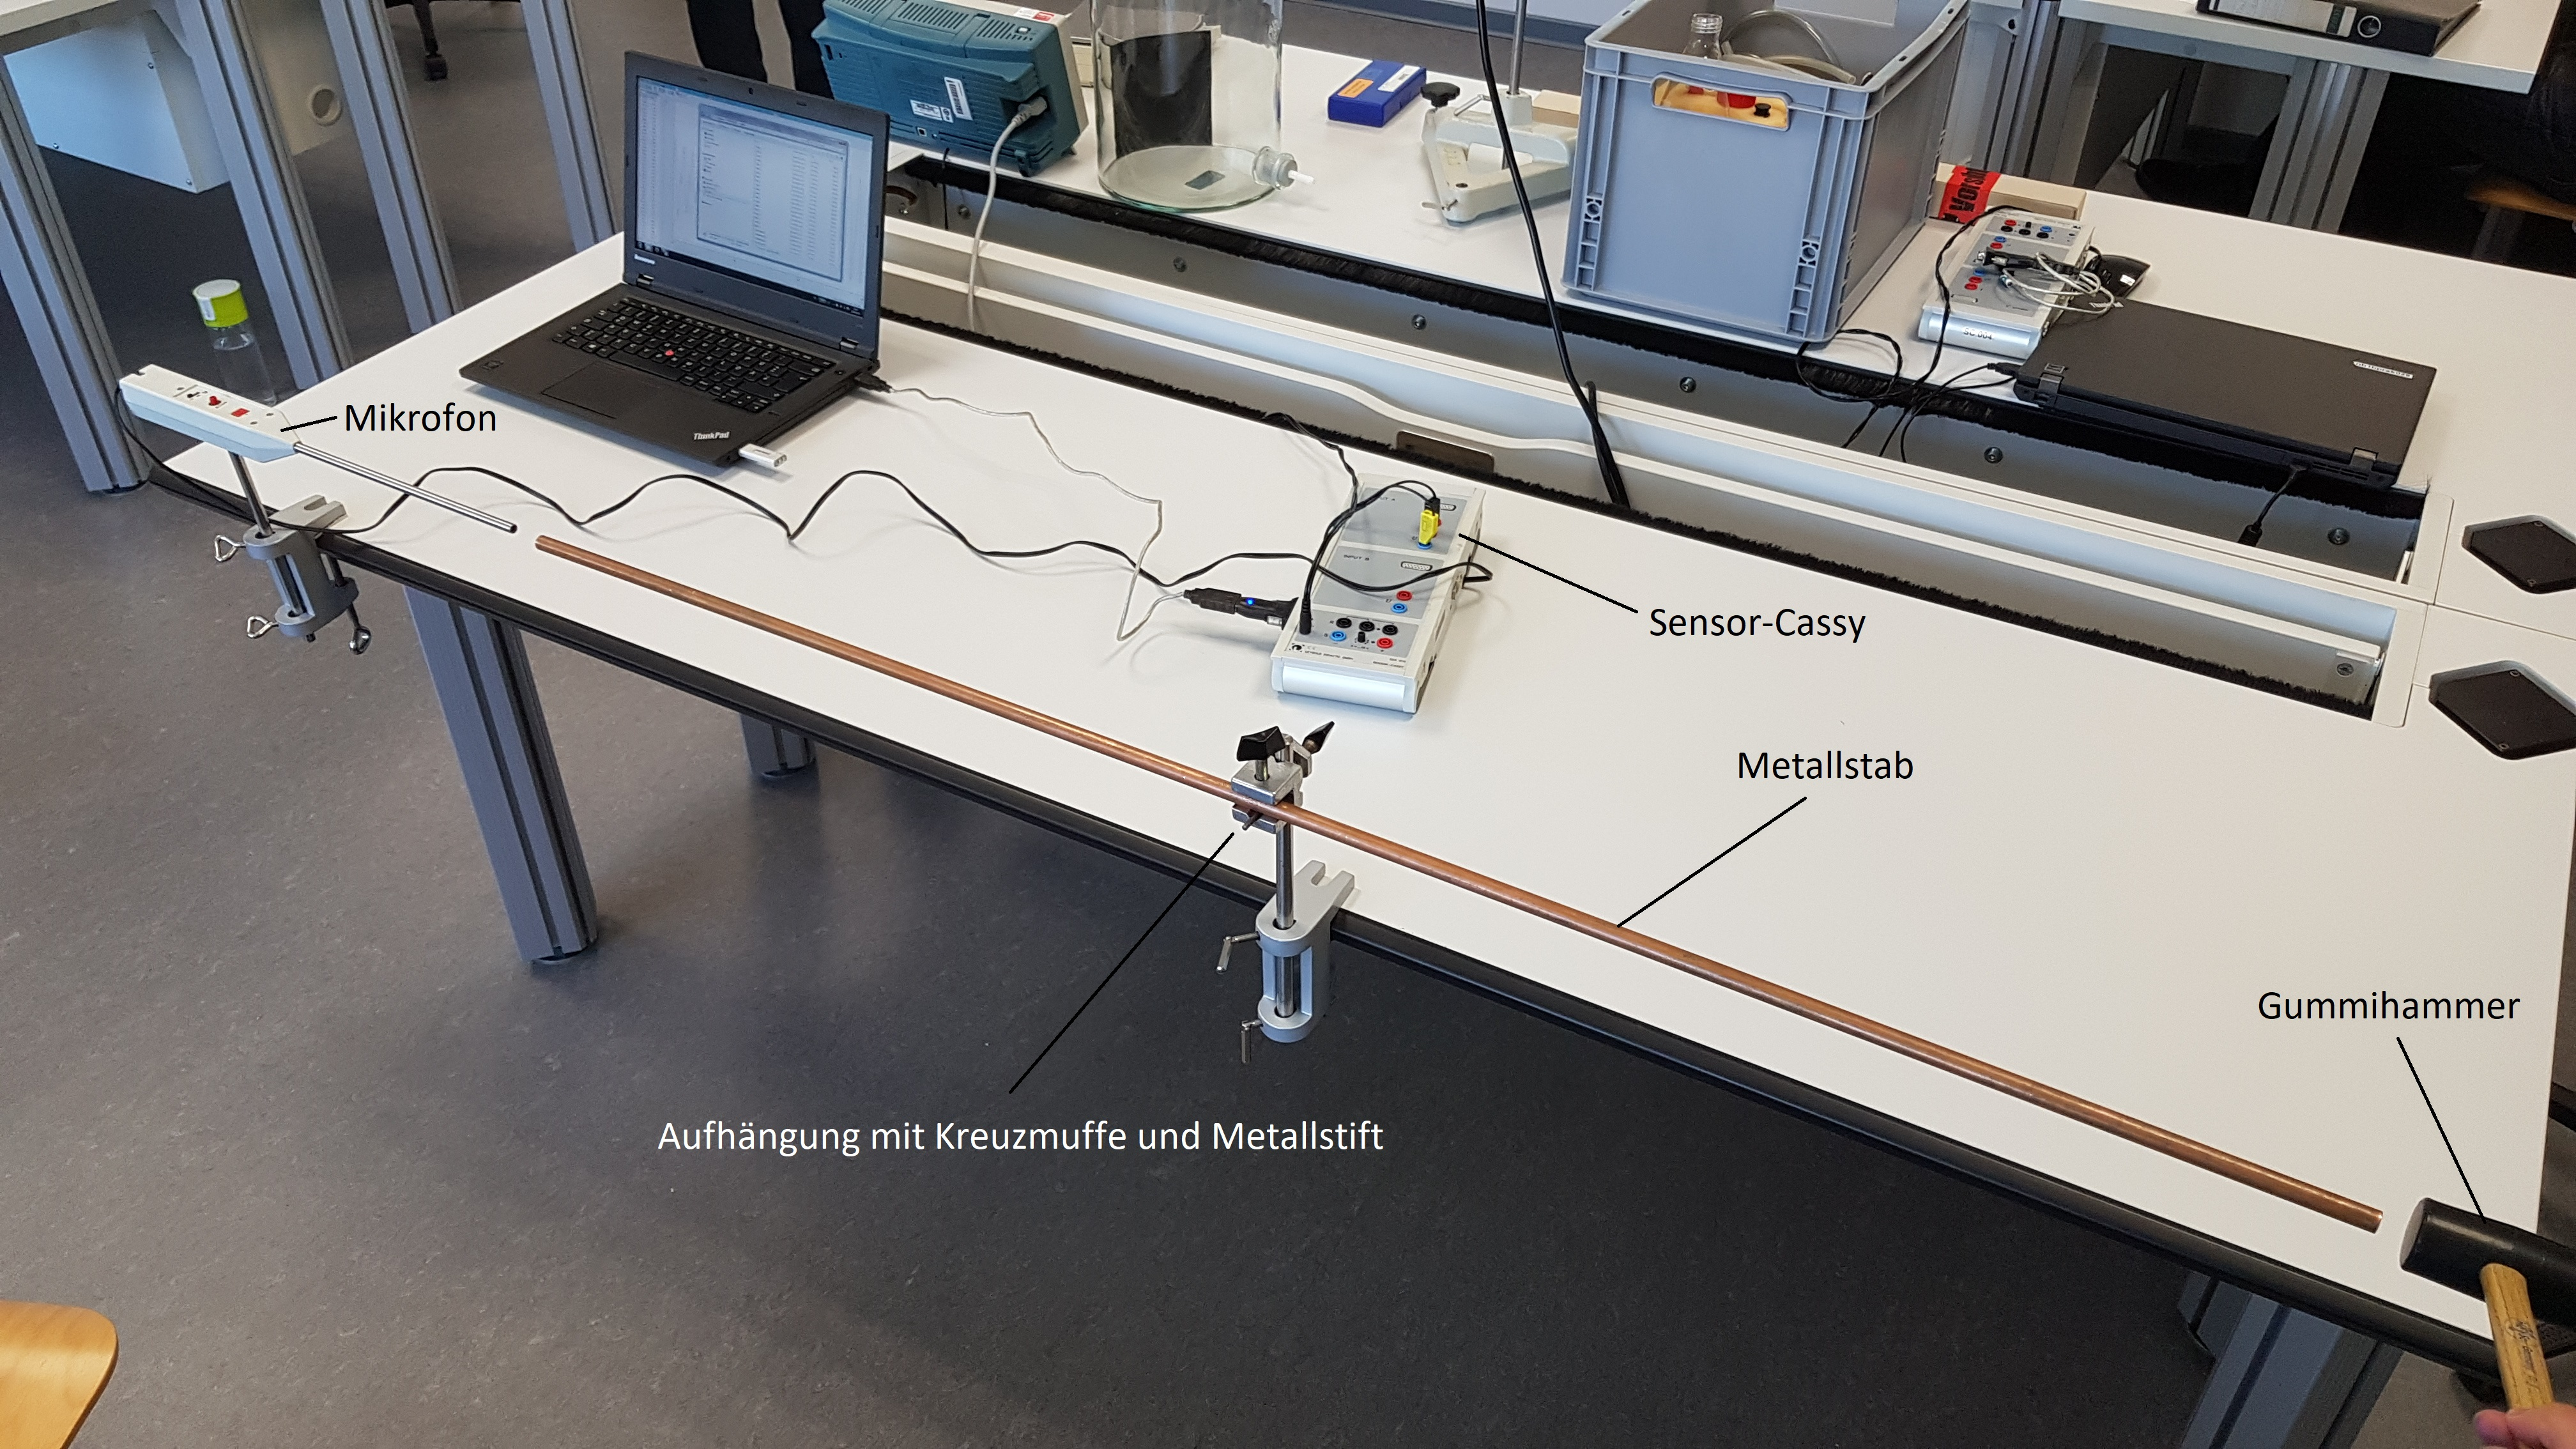
\includegraphics[width=\linewidth]{bilder/aufbau_festkoerper.jpg}
	\caption{Versuchsaufbau}
\end{figure}

Eine große, zu untersuchende Metallstange wird mit Hilfe einer Tischklemme, der kleinen Metallstange und der Kreuzmuffe horizontal am Tisch befestigt. Dabei muss die Stange mittig an zwei Punkten eingespannt werden, damit die Schwingung nicht beinträchtigt wird. Dies ist in Abbildung \ref{pic:aufhaengung} dargestellt. In kleinem Abstand zu einem Ende der großen Metallstange wird das Mikrofon platziert, das den Schalldruck und somit die Schallwellen misst. Das Mikrofon ist am Sensor-Cassy angeschlossen. Am anderen Ende kann die Stange durch einen Schlag mit dem Gummihammer in Schwingung versetzt werden.

\begin{figure}[H]
	\centering
	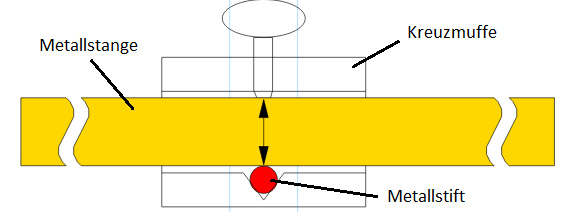
\includegraphics{bilder/aufhaengung_beschriftet.png}
	\caption{Aufhängung der Metallstange an zwei Punkten mit der Kreuzmuffe und einem Metallstift}
	\label{pic:aufhaengung}
\end{figure}



\subsection{Versuchsdurchführung}

Die Stäbe werden nacheinander ausgemessen und in die Versuchsvorrichtung eingespannt. Für die Länge wird das Maßband verwendet und für die Masse die Waage. Um den Durchmesser zu bestimmen, wird mit einer Mikrometerschraube an verschiedenen Stellen mit verschiedenen Orientierungen gemessen, da der Durchmesser variieren und eine Elliptizität nicht ausgeschlossen werden kann. Ist der Stab eingespannt und das Mikrofon eigeschaltet und ausgerichtet, kann der Stab durch einen Schlag mit dem Gummihammer in Schwingung versetzt werden. Der Schlag sollte möglichst gerade auf das Ende der Stange erfolgen, um transversale Schwingungen des Stabes zu vermeiden. Für jeden Stab wird die Messung fünfach durchgeführt. Bei den vorliegenden Messungen für die Stäbe 5 (Kupfer), 6 (Messing) und 9 (Aluminium) hatte das Seonsor-Cassy die Messparameter:
\begin{enumerate}[-]
\item Messbereich: $-3$ bis $3\,$V
\item Intervall: $100\,\mu$s
\item Messungen: $16000$
\item Messzeit: $1.6\,$s
\end{enumerate}
Da die gemessene Schwingung des Stahlstabes deutlich schneller abgeklungen ist als die der anderen Stäbe, wurden für die Messungen bei Stab 11 (Stahl) die Messparameter
\begin{enumerate}[-]
\item Messbereich: $-3$ bis $3\,$V
\item Intervall: $50\,\mu$s
\item Messungen: $16000$
\item Messzeit: $0.8\,$s
\end{enumerate}
verwendet.

\subsection{Versuchsauswertung}

Für die Messungen der Längen und Massen ergaben sich folgende Werte:

\begin{table}[H]
\centering
\begin{tabular}{cc|c|c|c}
Stabnummer & Material & $L$ [cm] & $M$ [g] & $\overline{D}$ [mm] \\
\hline
$5$ & Kupfer & $129.90\pm 0.07$ & $1295.00\pm 0.03$ & $11.991 \pm 0.081$ \\
$6$ & Messing & $130.00 \pm 0.07$ & $1237.20 \pm 0.03$ & $11.978 \pm 0.005$ \\
$9$ & Aluminium & $129.90 \pm 0.07$ & $407.30 \pm 0.03$ & $11.944 \pm 0.031$ \\
$11$ & Stahl & $130.10 \pm 0.07$ & $1157.60 \pm 0.03$ & $11.989 \pm 0.045$
\end{tabular}
\caption{Ergebnisse der Längen- und Massenmessungen}
\end{table}
Als Fehler in $\overline{D}$ wurde die Wurzel der empirischen Varianz und nicht die Standardabweichung des arithmetischen Mittels genommen, weil diese den Unebenheiten des Stabes nicht gerecht wird. In Abbildung \ref{pic:rohdaten} ist eine Messung des für den Kupferstab abgebildet.

\begin{figure}[h]
	\centering
	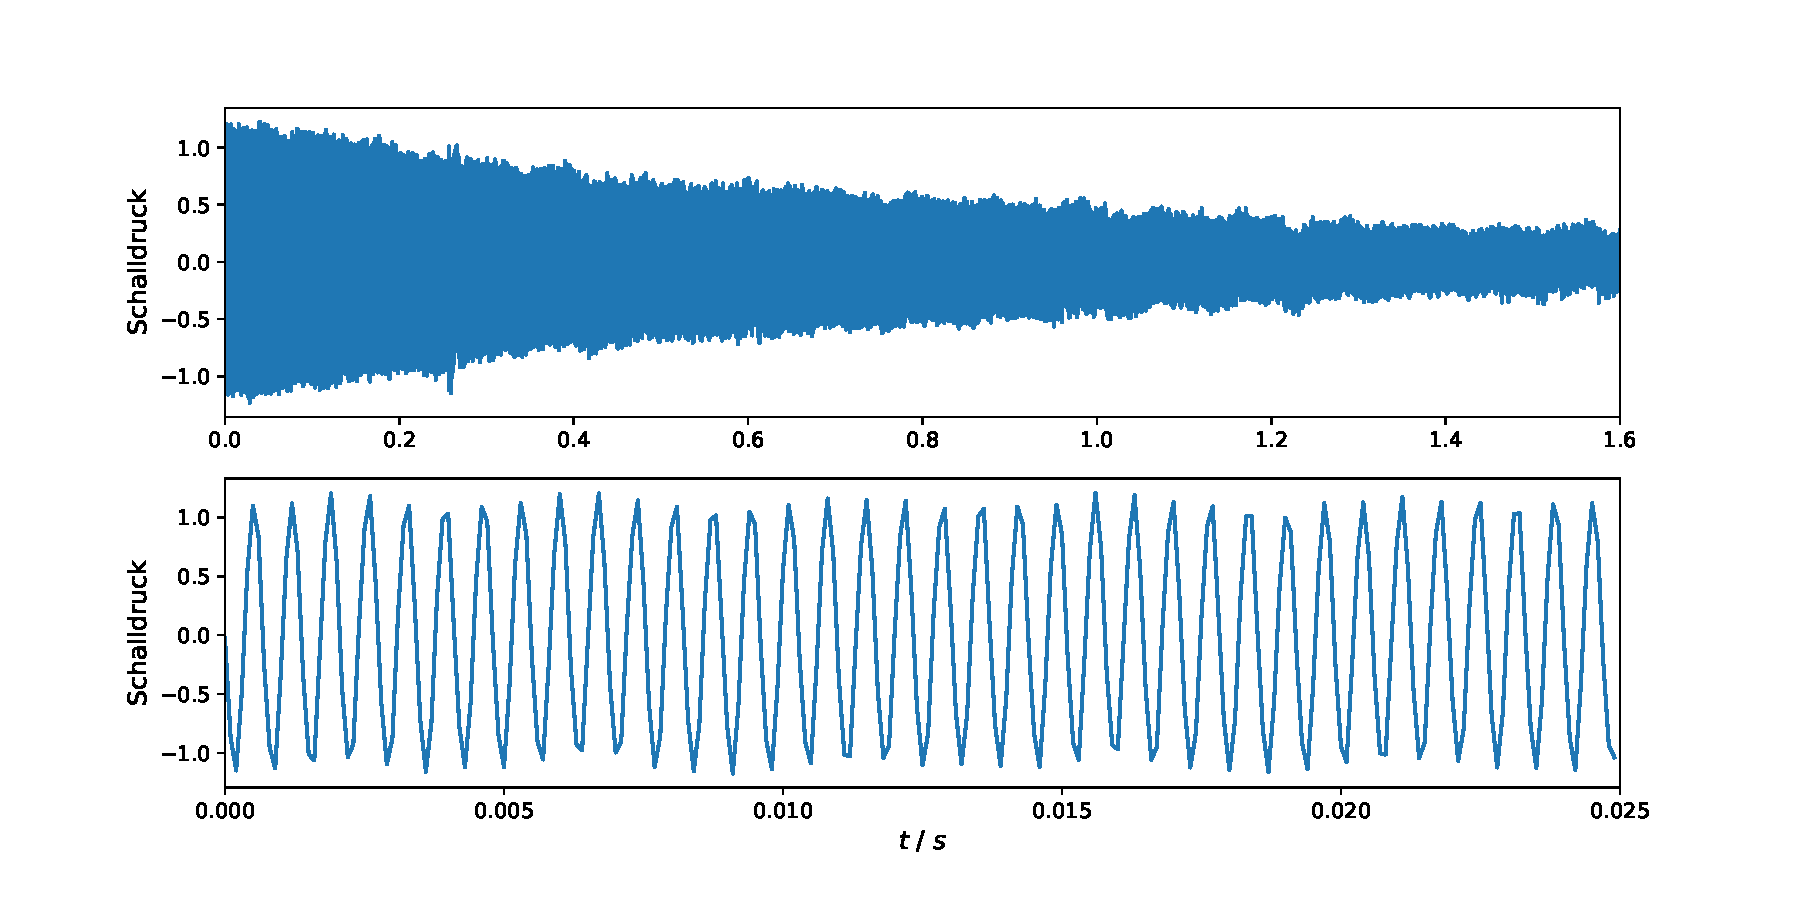
\includegraphics[width=\linewidth]{plots/rohdaten.pdf}
	\caption{Visualisierung der Rohdaten aus der ersten Messung für Stab 5 (\mbox{``Nr5\_1.lab''}) mit zwei verschiedenen Zeitskalen.}
	\label{pic:rohdaten}
\end{figure}

Die Bestimmung von $f_0$ erfolgt mit Hilfe der Frequenzspektren, die durch eine FFT aus den Rohdaten berechnet wird. Das Spektrum für die Schwingung aus Abbildung \ref{pic:rohdaten} ist beispielhaft in Abbildung \ref{pic:spektrum1} dargestellt. Man sieht deutlich die Grundschwingung bei circa $1500$Hz.

\begin{figure}[H]
	\centering
	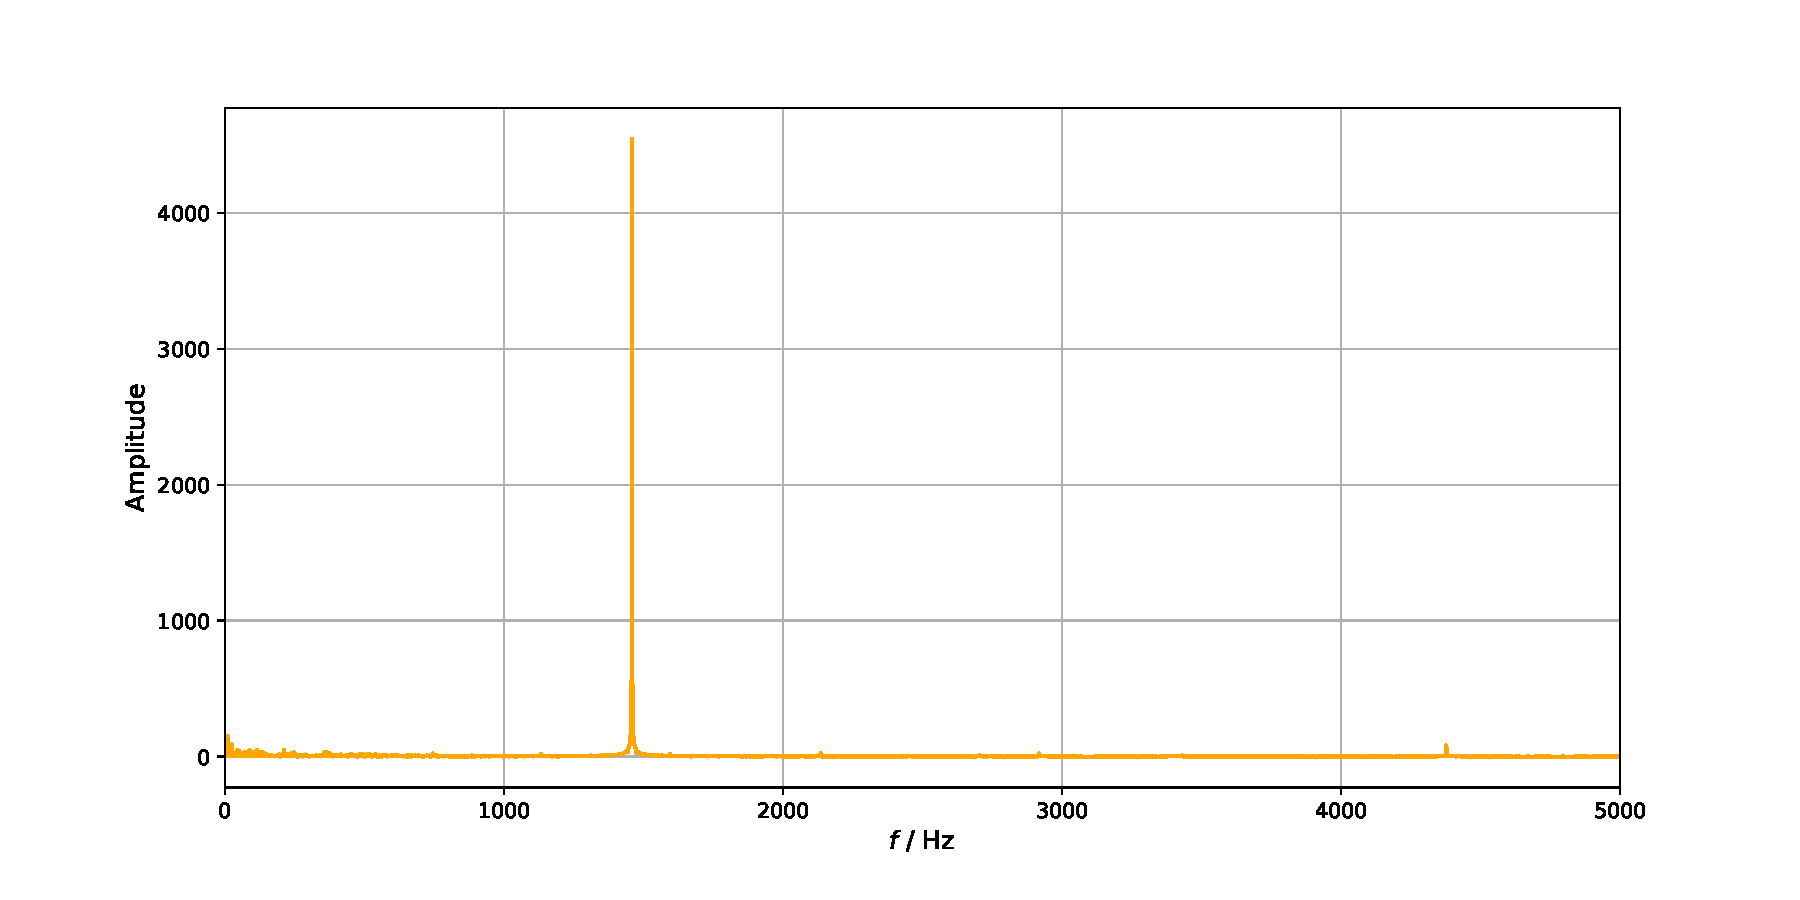
\includegraphics[width=\linewidth]{plots/spektrum1.pdf}
	\caption{Visualisierung des Spektrums der ersten Messung für Stab 5 (\mbox{``Nr5\_1.lab''}) berechnet mittels FFT.}
	\label{pic:spektrum1}
\end{figure}

Um $f_0$ möglichst exakt aus diesem Spektrum ablesen zu können, wird die Peakfinder-Methode aus dem Praktikumspaket verwendet. Für das Spektrum in Abbildung \ref{pic:spektrum1} ist dies in Abbildung \ref{pic:spektrum2} visualisiert. Im Anhang \ref{anhang:plot} finden sich für alle Messungen entsprechende Plots. Als Fehler, der durch das Ablesen, durch die FFT und durch Messunsicherheiten verursacht wird, wird $\sigma_{f} = 0.5\,$Hz verwendet.

\begin{figure}[H]
	\centering
	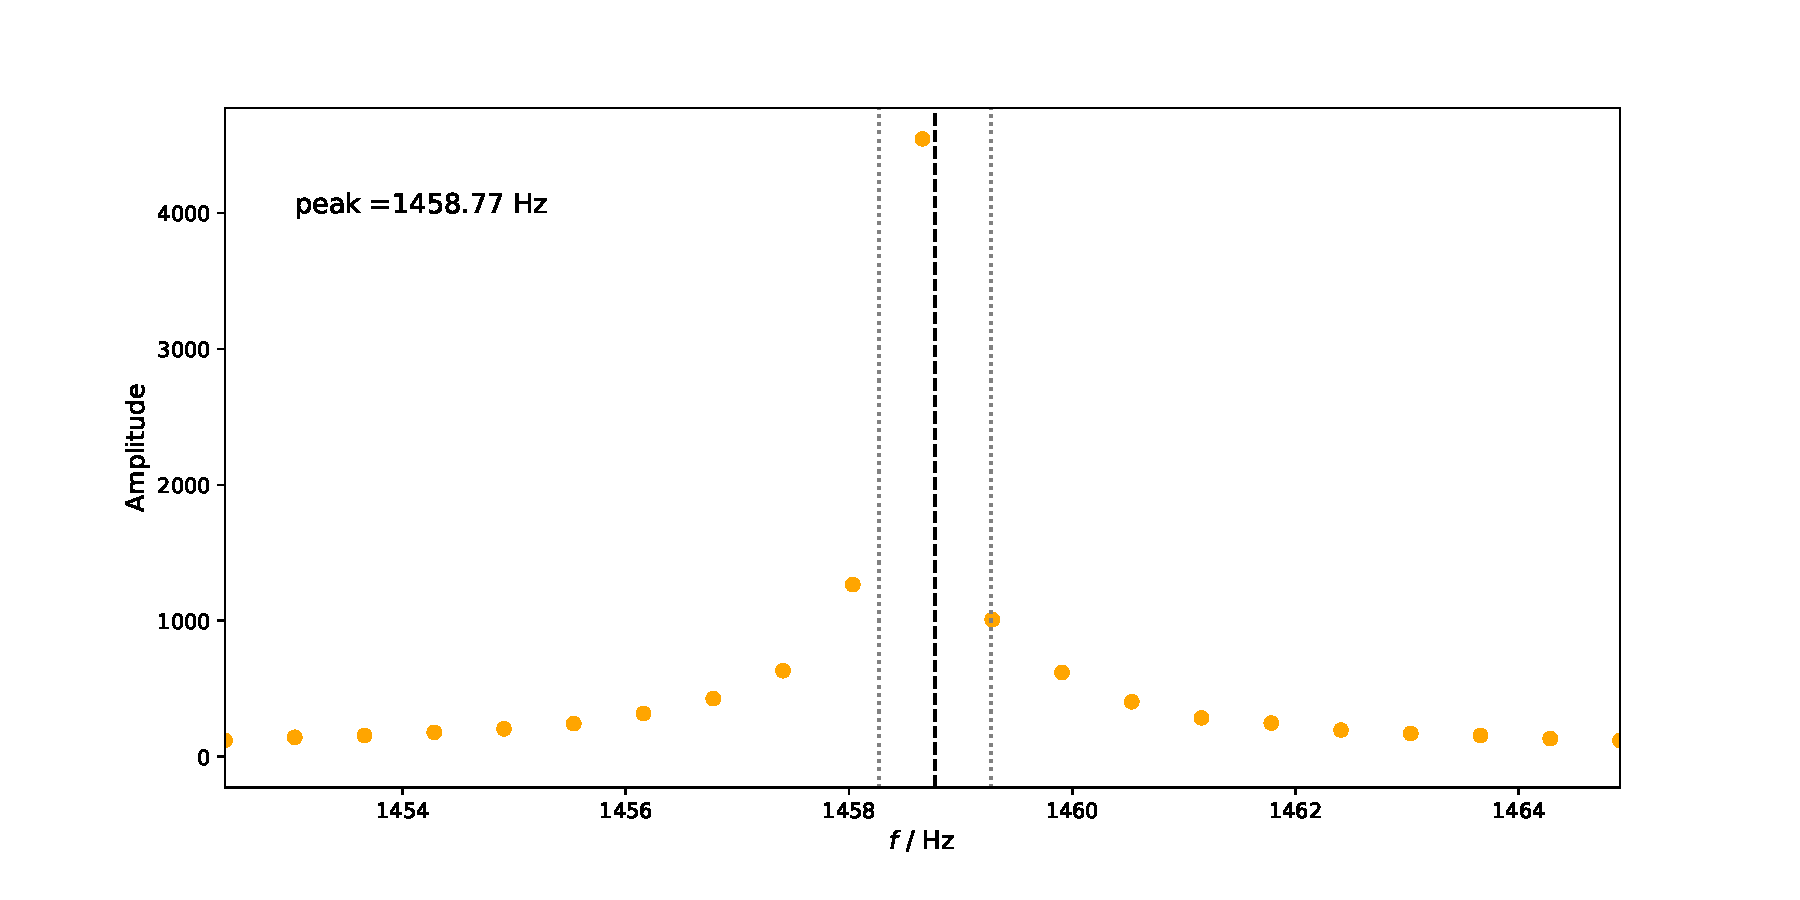
\includegraphics[width=\linewidth]{plots/spektrum2.pdf}
	\caption{Eingezeichnetes Ergebnis der Peakfinder-Methode (in schwarz) mit $\pm0.5\,$Hz (in grau) für das Spektrum der ersten Messung, Stab 5 (\mbox{``Nr5\_1.lab''}).}
	\label{pic:spektrum2}
\end{figure}

Daraus ergeben sich die folgenden Grundfrequenzen:

\begin{table}[H]
\centering
\begin{tabular}{cc|c}
Stabnummer & Material & $\overline{f}_0$ [Hz]\\
\hline
$5$ & Kupfer & $1458.810\pm 0.224$ \\
$6$ & Messing & $1348.122\pm 0.224$\\
$9$ & Aluminium & $1966.334\pm 0.224$\\
$11$ & Stahl & $1883.954\pm 0.224$
\end{tabular}
\end{table}
Zusammen mit den ermittelten Werten von $M$, $L$ und $\overline{D}$ lässt sich mit den Gleichungen \ref{eq:rho}, \ref{eq:ges} und \ref{eq:ela} die Dichte $\rho$, die (longitudinale) Schallgeschwindigkeit $v_l$ und das Elastizitätsmodul $E$ berechnen:

\begin{table}[H]
\centering
\begin{tabular}{cc|c|c|c}
Stabnummer & Material & $\rho$ [g/$\text{cm}^3$] & $v_l$ [m/s] & $E$ [N/$\text{m}^2$] \\
\hline
$5$ & Kupfer & $8.828\pm 0.118$ & $3789.988\pm 0.582$ & $(1.288\pm 0.017)\cdot 10^{11}$ \\
$6$ & Messing & $8.446\pm 0.006$ & $3505.117\pm 0.582$ & $(1.038\pm 0.001) \cdot 10^{11}$\\
$9$ & Aluminium & $2.798\pm 0.015$ & $5108.536\pm 0.582$ & $(0.730\pm 0.004)\cdot 10^{11}$\\
$11$ & Stahl & $7.882\pm 0.059$ & $4902.048\pm 0.582$ & $(1.894\pm 0.015)\cdot 10^{11}$
\end{tabular}
\end{table}

\subsection{Fazit}

Wir haben nun zwei Schätzungen für die Erdbeschleunigung $g$ ermittelt. Wie im Fazit des zweiten Versuchs erläutert, verwenden wir als Literaturwert für die Erbeschleunigung in Aachen $g_L = 9.811 \, \mathrm m / \mathrm s^2$. 
Zur Bewertung der beiden Ergebnisse berechnen wir
\begin{align*}
\frac{|g_L-g_{Dz}|}{\sigma_{g_{Dz}}} &= 0.12 \\
\frac{|g_L-g_{Os}|}{\sigma_{g_{Os}}} &= 1
\end{align*}
In beiden Fällen liegen wir somit im $1\sigma$-Intervall. Zur Überprüfung der Übereinstimmung der beiden Werte untereinander berechnen wir noch
$$\frac{|g_{Os}-g_{Dz}|}{\sqrt{\sigma_{g_{Dz}}^2 + \sigma_{g_{Os}}^2}} \approx 0.03 \ll 1.$$
Die beiden Werten stimmen also im Rahmen der Unsicherheiten sehr gut überein. 


\newpage


\appendix
\newpage
\section{Ergebnisse der Peakfinder-Methode}\label{anhang:plot}
\begin{figure}[H]
	\centering
	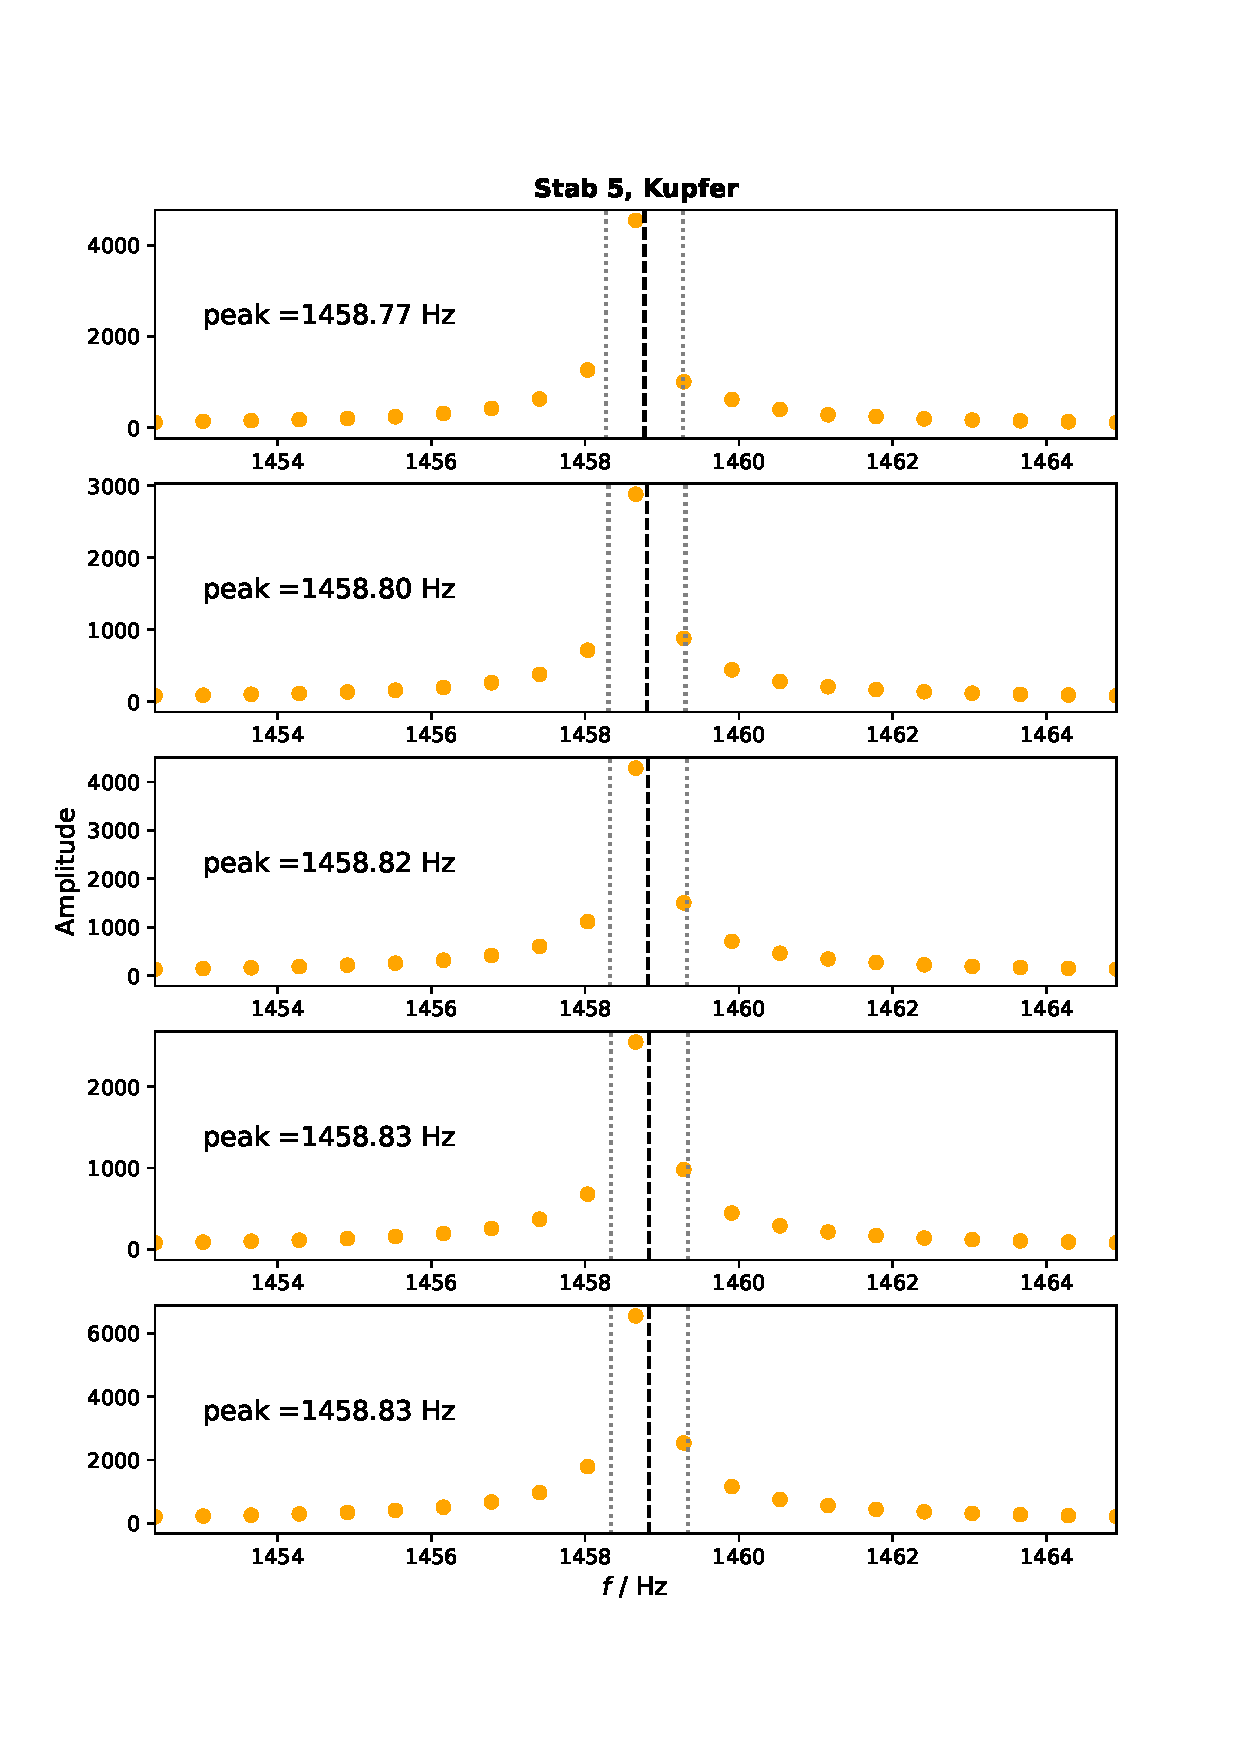
\includegraphics[width=\linewidth]{plots/anhang1.pdf}
\end{figure}

\begin{figure}[H]
	\centering
	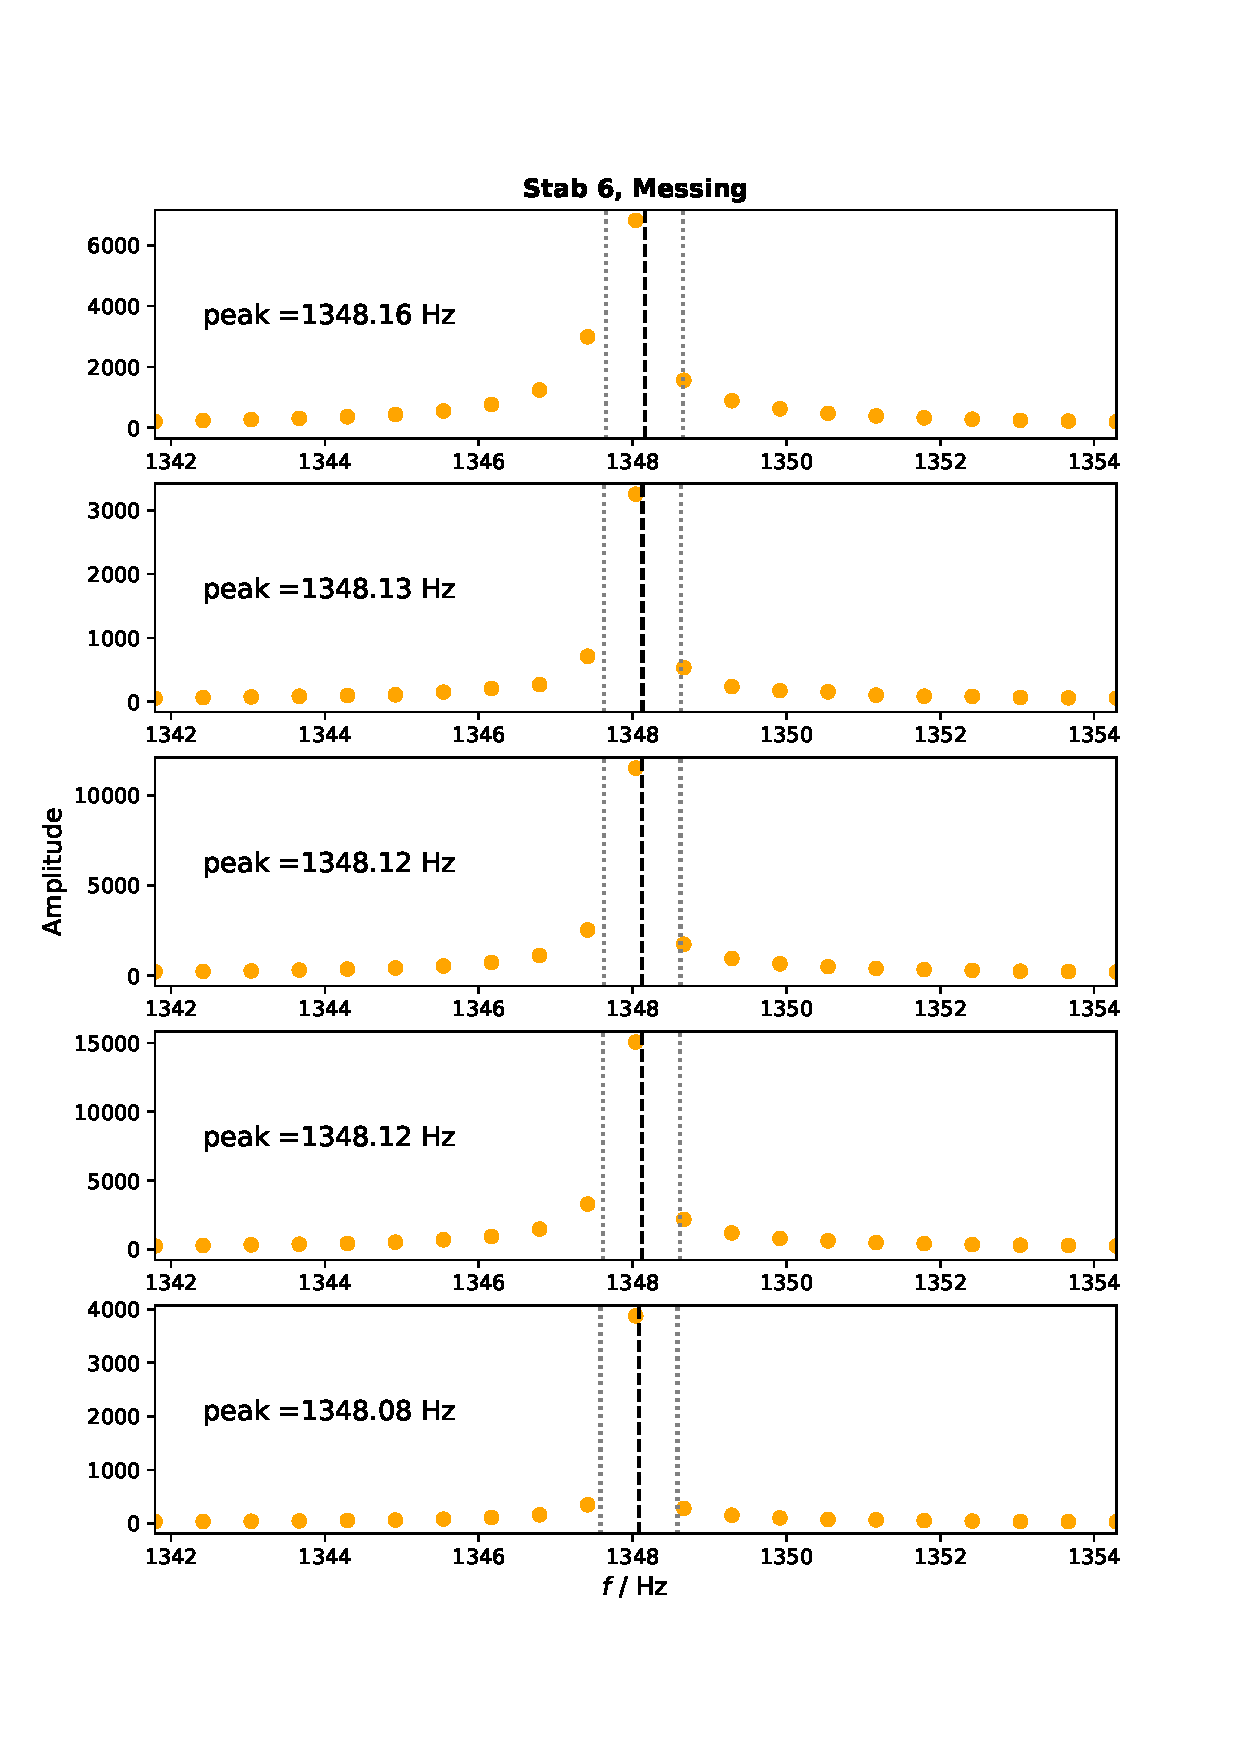
\includegraphics[width=\linewidth]{plots/anhang2.pdf}
\end{figure}

\begin{figure}[H]
	\centering
	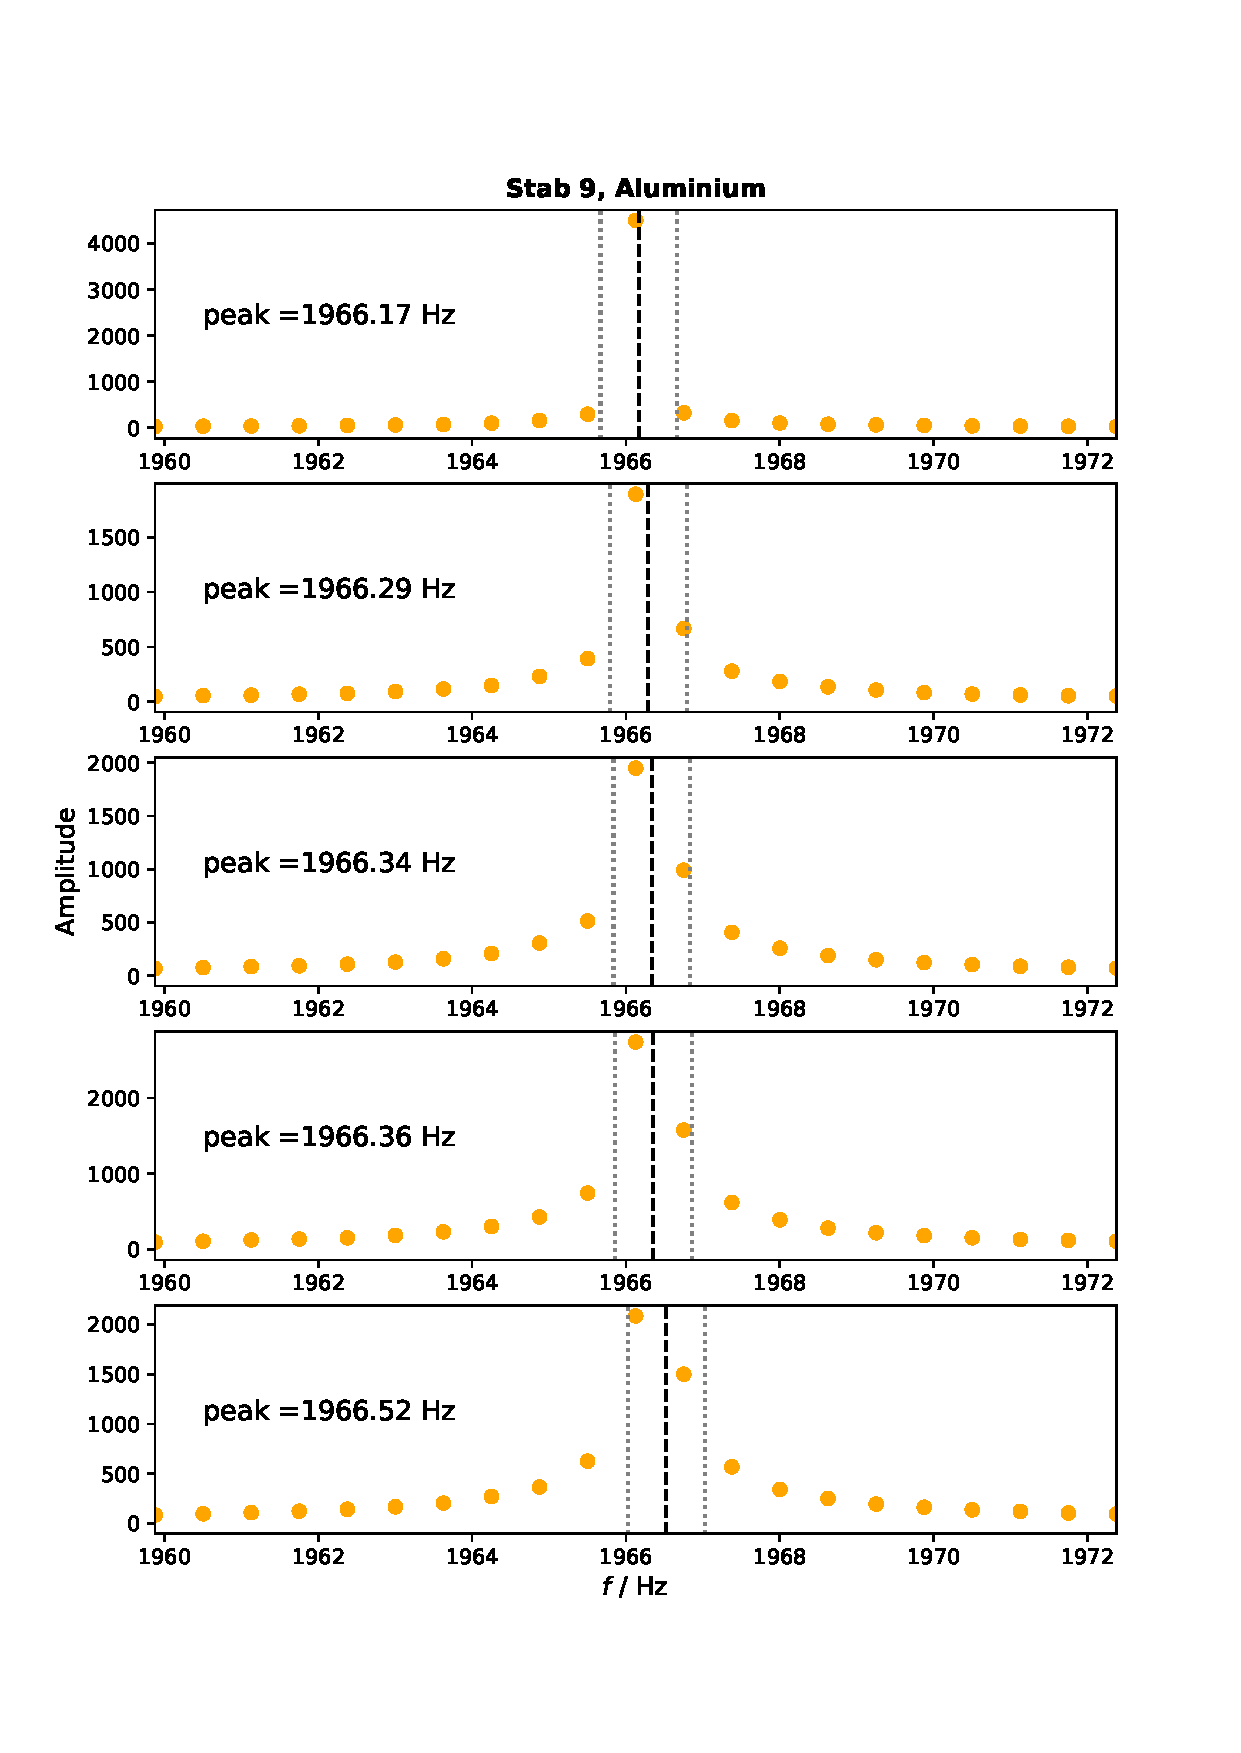
\includegraphics[width=\linewidth]{plots/anhang3.pdf}
\end{figure}

\begin{figure}[H]
	\centering
	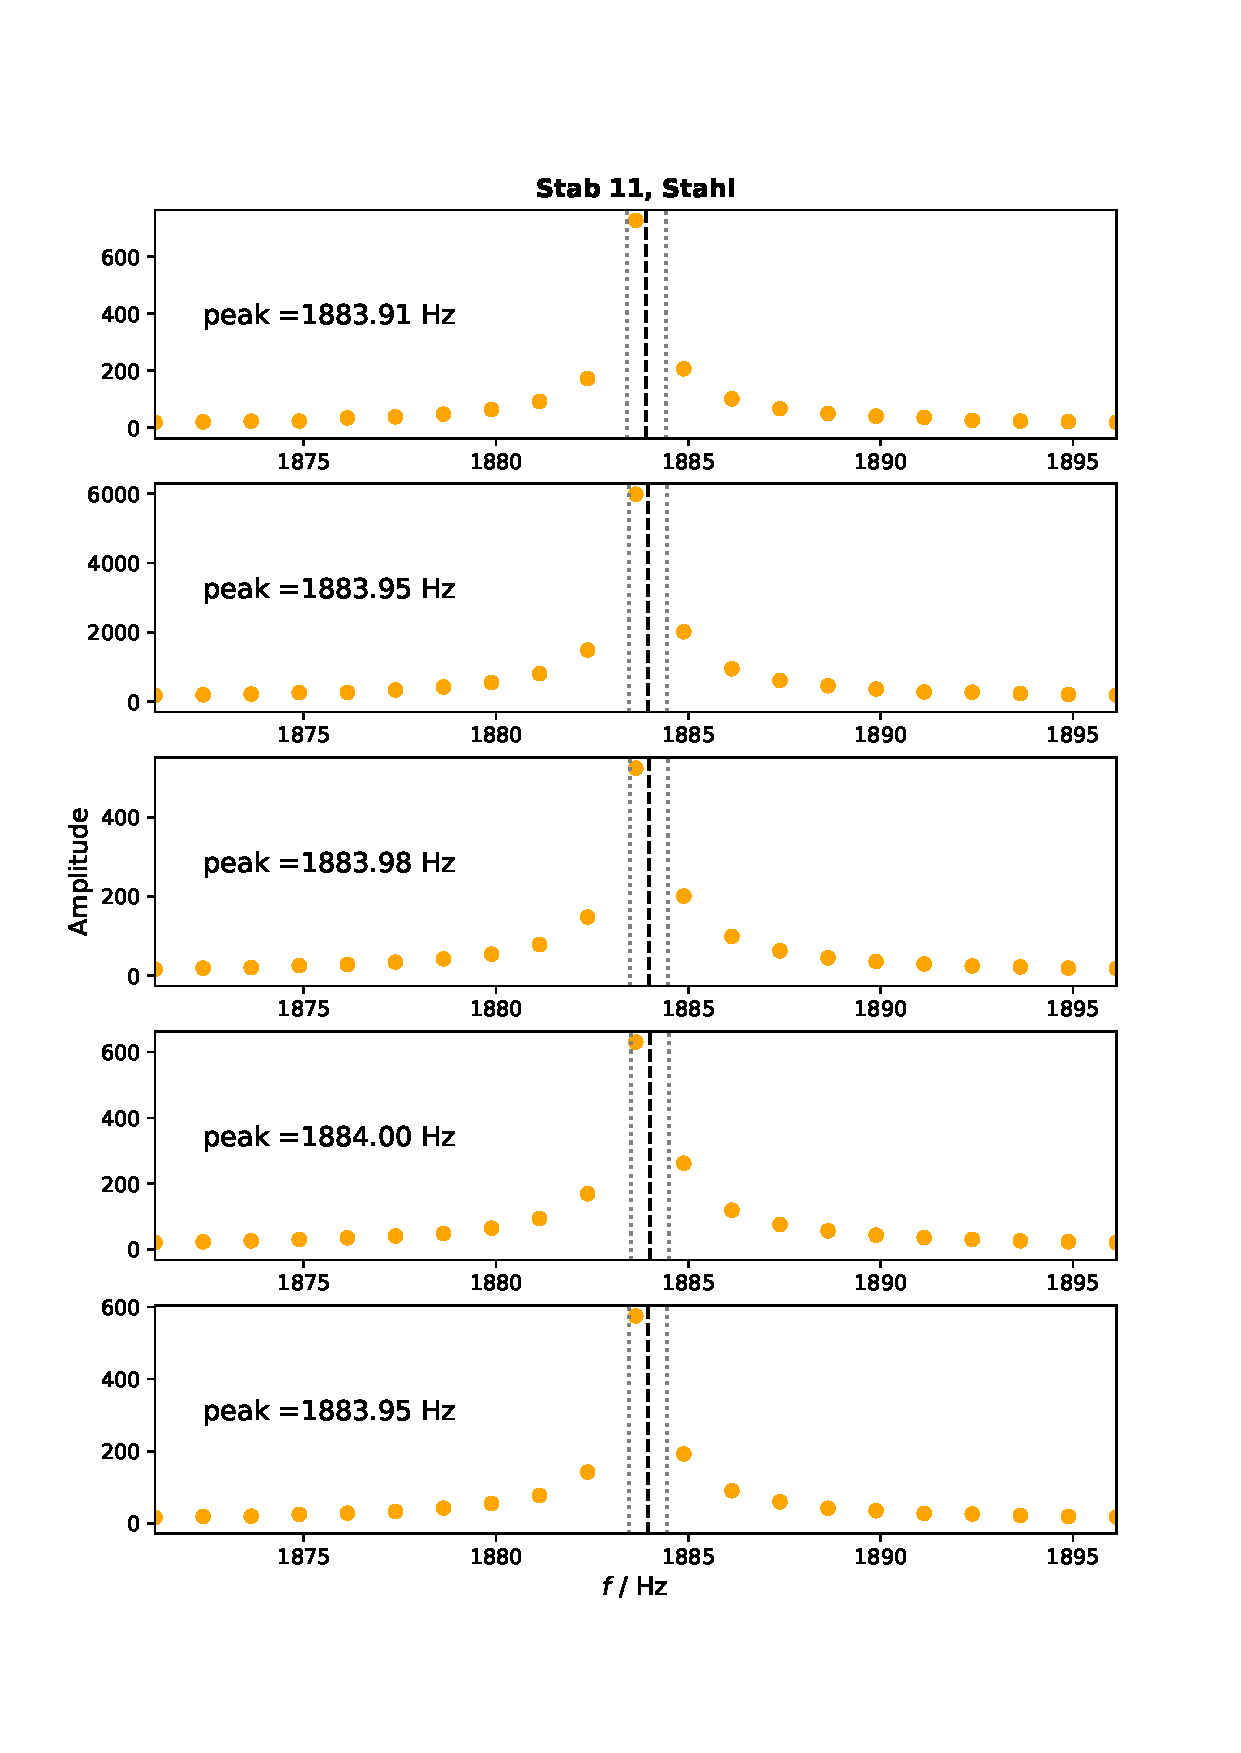
\includegraphics[width=\linewidth]{plots/anhang4.pdf}
\end{figure}


\end{document}
